\documentclass[a4paper]{article}
\usepackage[utf8]{vietnam}
\usepackage{graphicx}
\usepackage{amsfonts}
\usepackage{amssymb}
\usepackage{mdsymbol}
\usepackage{amsmath}
\usepackage[linesnumbered,ruled]{algorithm2e}
\usepackage[top=2cm, bottom=2cm, left=2cm, right=2cm]{geometry}
\usepackage{comment} % enables the use of multi-line comments (\ifx \fi) 
\usepackage{lipsum} %This package just generates Lorem Ipsum filler text. 
\usepackage{fullpage} % changes the margin
\setlength{\parindent}{0pt}

\usepackage{filecontents}
\usepackage[numbers]{natbib}
\graphicspath{{./}}	

\begin{document} 

\title{Improved Galactic Swarm Optimization}
\maketitle
\noindent

\section{Improved Galactic Swarm Optimization (IGSO)}
GSO is a global optimization metaheuristic based on the ideas of swarm optimization algorithms. GSO takes advantage of origin swam-based algorithms such as Particle Swarm Optimization (PSO) and Elephant Herding Optimization (EHO) by using flexibly mutiple cycles of exploration and exploitation phases to escape local minimums and land to new better solutions. Apart from   this advantage, the PSO algorithms used in 2 phases of original GSO, however, cause a porverty of exploitation and exploration that leads to a mediocre convergence. In this paper, another swarm-based optimization called Levyflight-based Whale Optimization Algorithm (Levyflight WOA) is chosen instead of PSO to tackle problem mentioned above. 
\subsection{Galactic Swarm Optimization (GSO) Standard}
The GSO algorithm has an inspiration from the behaviours of stars in galaxies, and of galaxies in superclusters of galaxies in the cosmos. Under the influence of gravity, stars in a galaxy are attracted to another star which have greater gravity. That means they are likely to follow the bigger star in a galaxy, and the same phenomena happens to galaxies in supercluster galaxies. From these ideas, movement of stars inside a galaxy as well as movement of galaxies is emulated in GSO algorithm by following rules: Firstly, individuals in each galaxy are attracted to the better solutions in the galaxy using PSO algorithm. Secondly, global bests of all galaxies are chosen to represent galaxies and treated as a superswarm. PSO algorithm is used again to present the movement of particles in superswarm. \\
The original GSO was first presented in ......, and the skeleton of this algorithm is given in Algorithm 1 with two main below-describe parts.  \\


\textbf{Part 1:} Initialize GSO parameters and population. \\
The main control parameters of whole GSO algorithm consist of GSO parameters and PSO parameters used in each phase. \textbf{Table 1} shows the detail of all parameters in GSO algorithm. \\
Population, or swarm, consists of M partitions called subswarms $X_i$ containing N elements ($x_j^{(i)}\in$ $\mathbb{R}^D$). Each element is created randomly within the search space $[x_{min}, x_{max}]^D$. After initialization is finished, the complete swarm of GSO algorithm is as follow: \\ \\
$X = \left\{X_i|  i = 1, 2, ..., M\right\}$ \\ \\
$X_i = \left\{X_j^{(i)}|   j = 1, 2, ..., N\right\}$ \\ \\
$X_i\cap X_j = \varnothing$ $  \forall i != j $ \\ \\
$X_i$ is a swarm of size N. Velocity and personal best tied to particle $x_j^{(i)}$ are denoted as $v_j^{(i)}$ and $p_j^{(i)}$ respectively. Each subswarm $X_i$ is associated to a global best known as $g^{(i)}$ which is later a particle in superswarm Y. See more in \textbf{Table 1}. \\
\begin{tabular}{ |p{3cm}||p{9cm}| }
 \hline
 \multicolumn{2}{|l|}{\textbf{Table 1:} Parameters in GSO}  \\
 \hline
 \textit{Parameters}& \textit{Meaning}\\
 \hline
 $f$   & Cost function   \\
 $X$   & Population consists of all particles $x_j^{(i)}$ in the swarm \\
 $D$   & Dimension of a solution \\
 $X_i$ & subset of population belonging to subswarm $i$ \\
 $x_j^{(i)}$  & position of particle $j$ in subswarm $i$ \\
 $v_j^{(i)}$  & Velocity of particle $x_j^{(i)}$ \\
 $p_j^{(i)}$  & Personal best of particle $x_j^{(i)}$ \\
 $g^{(i)}$  & Global best of subswarm $i$ \\
 $y^{(i)}$  & position of particle i in superswarm (current global best of subswarm $i$) \\
 $v^{(i)}$  & Velocity of $y^{(i)}$ \\
 $g$  & Global best solution of superswarm \\
 $Iteration_{max}$  & number of iterations \\
 $M$  & Number of subswarms \\
 $N$  & Size of subswarm $i$ \\
 $L_i$  & Number of iterations in phase i \\
 $c_1, c_2, c_3, c_4$  & Acceleration coefficient of PSO used in 2 phases \\
 $r_i$  & Uniform distributed random number in $[-1, 1]$ \\
 $w_i$  & Inertial weight \\
 
 \hline
\end{tabular}
\\ \\

\textbf{Part 2:} Exploration and exploitation by PSO algorithm.This part includes two phases represented in following steps: \\ \\
\textit{$(1)$ Phase 1: Exploration of subswarms} \\
PSO algorithm is run for each subswarm. Since swarm $X$ initially divided into $M$ groups, PSO will run for $M$ times independently with global bests $g^{(i)}$ tied to each subswarm. $g^{(i)}$ will be updated if any particles in the subswarm have personal best $p_j^{(i)}$ which is a better solution than $g^{(i)}$,  $f(p_j^{(i)}) < f(g^{(i)})$. \\
Each subswarm independently explores its best solution freely in its search space. This task begins following PSO algorithm by calculating velocity $v_j^{(i)}$ and position $x_j^{(i)}$ of particles. The formulas of calculation are: \\ \\
$v_j^{(i)}\gets\omega_1v_j^{(i)} + c_1r_1(p_j^{(i)} - x_j^{(i)}) + c_2r_2(g^{(i)} - x_j^{(i)})$ \\ \\
				$x_j^{(i)}\gets$ $x_j^{(i)} + v_j^{(i)}$ \\ \\
where the inertial weight $\omega_1$ and random number r1, r2 are described as:\\ \\
$\omega_1 = \frac{Iteration_{max} - Iteration}{Iteration_{max}}*(w_{max} - w_{min}) + w_{min}$ \\ \\
$r_i = U(-1, 1)$ \\ \\
$Iteration$ is the current epoch, while $w_{max}$ and $w_{min}$ are boundary of $\omega_1$. The second formula means that $r_i$ is a random number uniformly distributed in range $[-1, 1]$. \\ \\
\textit{$(2)$ Phase 2: Exploitation in superswarm} \\
All global bests from M subswarms in \textit{phase 1} are gathered together to form the superswarm. New superwswarm $Y$ is created by collecting M global bests of each subswarm $X_i$. \\ \\
$Y = \left\{y^{(i)}| y^{(i)} = g^{(i)}, \forall i = 1, 2, ..., M\right\}$ \\ \\
The velocity $v^{(i)}$ and the position $y^{(i)}$ are updated by the equations given below: \\ \\
$v^{(i)}\gets\omega_2v^{(i)} + c_3r_3(p^{(i)} - y^{(i)}) + c_4r_4(g - y^{(i)})$ \\ \\
				$y^{(i)}\gets$ $y^{(i)} + v^{(i)}$ \\ \\
where $p^{(i)}$ is the personal best of particle $y^{(i)}$, and parameters $\omega_2, c3, c4, r3, r4$ brought here with the same meaning to parameters in \textit{phase 1}. $g$ is the global best of the entire population and not be updated unless a better point is found. \\
The superswarm utilizes the best solutions already computed by subswarms, and then analyzes and exploits information from each best solution. Considering that the global bests of subswarms influence the superswarm, but there is no feedback or information flow back from superswarm to subswarms for conserving the diversity of population. Superswarm is newly created every epoch, then it exploits information and considers nothing more than global best of population $g$. When a new epoch starts, the search of subswarms starts from exactly where they left off. It means that the subswarms do not get started from beginning. The \textbf{Algorithm 1} shows the pseudo-code of GSO algorithm. \\ \\ 
\begin{algorithm}[H]
\SetAlgoLined
 initialization: $x_j^{(i)}$, $v_j^{(i)}$, $p_j^{(i)}$, $g_j^{(i)}$, within $[x_{min}, x_{max}]^D$ randomly. \\
 initialization: $v^{(i)}, p^{(i)}, g$ within $[x_{min}, x_{max}]^D$ randomly. \\
 \For{$Iteration\gets0$ to $Iteration_{max}$}
 {
 	Begin PSO: Level 1 \\
	\For{$i\gets1$ to $M$}
	{
		\For{$k\gets0$ to $L_1$}
		{
			\For{$j\gets1$ to $N$}
			{
				$v_j^{(i)}\gets\omega_1v_j^{(i)} + c_1r_1(p_j^{(i)} - x_j^{(i)}) + c_2r_2(g^{(i)} - x_j^{(i)})$; \\
				$x_j^{(i)}\gets$ $x_j^{(i)} + v_j^{(i)}$; \\
				\If {$f(x_j^{(i)}) < f(p_j^{(i)})$}
				{
					$p_j^{(i)}\gets$ $x_j^{(i)}$; \\
					\If {$f(p_j^{(i)}) < f(g^{(i)})$}
					{
						$g^{(i)}\gets$ $p_j^{(i)}$;
					}
				}
			}
		}
	}
	Begin PSO: Level 2 \\
	Initialize Swarm $y^{(i)} = g^{(i)}: i = 1, 2, ..., M;$ \\
	\For{$k\gets0$ to $L2$}
	{
		\For{$i\gets1$ to $M$}
		{
			$v^{(i)}\gets\omega_2v^{(i)} + c_3r_3(p^{(i)} - y^{(i)}) + c_4r_4(g - y^{(i)})$; \\
			$y^{(i)}\gets$ $y^{(i)} + v^{(i)}$; \\
			\If {$f(y^{(i)}) < f(p^{(i)})$}
				{
					$p^{(i)}\gets$ $y^{(i)}$; \\
					\If {$f(p^{(i)}) < f(g)$}
					{
						$g\gets$ $p^{(i)}$;
					}
				}
			
		}
	} 	
 }
 \KwResult{$g, f(g)$}
 \caption{Galactic Swarm Optimization (GSO)}
\end{algorithm}
\subsection{Whale Optimization Algorithm (WOA) Standard}
Whales, which are known as the biggest mammals in the world, are interesting creatures. Depending on whales size, environment and their food, they are categorized into seven several species such as beluga whale, blue whale, bowhead whale, gray whale, killer whale and humpback whale. Different categories of whale have different methods for foraging which work effectively on their kinds of food. One of the biggest ballen whales is humpback whales. Adult humpback whales have length of $12-16m$ and weigh around $25-30$ metric tons. Their favorite prey are krill and small fish herds. \\
Considering the way humpback whales hunt their prey, it is amazing and interesting. This hunting activity is called bubble-net feeding which is often done in groups. The group size can range from two or three and up to sixty whales participating at once. The bubble net is form by launching vocalizations of a whale to communicate to the others. Once signals are received by other whales, they start to blow bubbles while continuing to surround their prey. Prey then is enclosed into the net and disoriented because of bubbles humpback whales release consecutively. After the bubble net is executed, it is kept shrinking until food is totally eaten. \\
From the idea of hunting strategy mentioned above of humpback whales, Whale Optimization Algorithm (WOA) was born to mimic the amazing social behaviors of these creatures. Analogous to bubble-net creation and execution, \textit{shrinking encircling mechanism} and \textit{spiral updating position} present perfectly foraging process executed by humpback whales. WOA was first introduced in .... The detail of this algorithm is presented in \textbf{Algorithm 2} with the following parameters and equations explanation part: \\ \\  
\textbf{Part 1: Encircling prey.} \\
Humpback whales in nature can locate their prey and start to surround them when a whale launch vocalizations. In WOA, however, the position of prey is not known at first because the whale population is initialized randomly. To handle this problem, WOA assumes that the solution with the best fitness will be the prey, and it is reset at the beginning of each iteration. After the target is recognized, other whales will try to update their position around the prey. This behavior is represented by following expressions: \\ \\
$D = |C.X^*(t) - X(t)|$ \\ \\
$X(t+1) = X^*(t) - A.D$ \\ \\
where $t$ is the current iteration, $A$ and $C$ are coefficients, $X^*$ is the position vector of solution known as the best, $X$ is the position of solution need to be updated, $|.|$ indicates absolute value and $.$ is an element-by-element multiplication. After each iteration, $X^*$ will be updated if a better solution is found. \\
The two coefficients $A$ and $C$ are defined as follows: \\ \\
$A = 2a.r_1 - a$ \\ \\
$C = 2.r_2$ \\ \\ 
where $a \in$ $[0,2]$ is linearly decreased following the increase of iteration, and $r1$, $r2$ are random numbers in $[0,1]$. \\
Different positions around the best solution can be obtained with respect to distance from the current position by adjusting the values  of $A$ and $C$. Additionally, by defining two random values $r1$ and $r2$, it is expected that solutions can reach any positions inside search space created by equations above. \\ \\
\textbf{Part 2: Bubble-net attacking method (exploitation phase).}\\
Two approaches are designed analogous to two behaviors of humpback whale swarm when they execute their bubble-net in nature:\\ \\
\textit{(1) Shrinking encircling mechanism:} \\
This mechanism is achieved by reducing the magnitude of $a$, and the value of $A$ is reduced following $a$. Considering that $A$ is a random value in $[-a,a]$ with linearly decreased a from $2$ to $0$. Considering that if $A \in$ $[-1,1]$, the updated position will surely be landed in the space between the orginal position of solution and the position of best solution in current iteration. \\ \\
\textit{(2) Spiral updating postion} \\
This operation is based on the way humpback whales approach their prey. A spiral equation is created to emulate the helix-shape movement of humpback whales within the space between the position of whale and prey: \\ \\
$X(t+1) = D'.e^{bl}.\cos(2\pi l) + X^*(t)$; \\ \\
where $D' = |X^*(t) - X(t)|$ indicates the absolute distance between current solution (current whale) and best solution (the prey), $b$ is a constant forming the shape of the spiral, and $l$ is a random number in $[-1,1]$. \\
The mathematical model is represented as follow: \\ \\
\[
    f(x)= 
\begin{cases}
    X(t+1) = X^*(t) - A.D,& \text{if } p\geq 0.5\\
    X(t+1) = D'.e^{bl}.\cos(2\pi l) + X^*(t),              & \text{otherwise}
\end{cases}
\]
where $p$ is a random number in $[0,1]$. Considering that whale approach their prey by swimming around within a shrinking circle and following a spiral path simultaneously. The point $p = 0.5$ means that both mechanisms have the same probability to happen. \\ \\
\textit{(3) Search for prey (exploration phase):} \\
In addition to the bubble-net method, whales search for prey randomly. In exploitation phases, particularly in \textit{Shrinking encircling mechanism}, new position is updated when $|A|\geq 1$, which makes whale come closer to prey. In contrast, if $|A| > 1$ searching for prey mechanism is presented as a random process of choosing a new solution. This process emphasizes exploration and allows WOA to escape local minimum easily. The mathematical model is as follow: \\ \\
$D \gets$ $|C.X_{rand} - X(t)|$ \\ \\
$X(t+1) \gets$ $X_{rand} - A.D$ \\ \\
where $X_{rand}$ is a random position vector chosen from current position. \\ \\

\begin{algorithm}[H]
\SetAlgoLined
 Initialize the whales population $X = \left\{X_i| i = 1, 2, ..., n\right\}$ within $[x_{min}, x_{max}]^D$ randomly. \\
 Calculate fitness of each solution (whale) \\
 $X^*\gets$ the best solution \\
 \For{$Iteration\gets0$ to $Iteration_{max}$}
 {
 	Begin updating positions: \\
 	\For{whale in population}
 	{
		Update parameters $a, A, C, l$ and $p$ \\ 	
		\eIf {$p < 0.5$}
		{
			\eIf{$|A| < 1$}
			{
				Shrinking encircling mechanism:\\
				$D \gets$ $|C.X^*(t) - X(t)|$; \\
				$X(t+1) \gets$ $X^*(t) - A.D$; \\
			}
			{	
				Search for prey (exploration phase):\\
				Select a random solution ($X_{rand}$) in current population; \\
				$D \gets$ $|C.X_{rand} - X(t)|$; \\
				$X(t+1) \gets$ $X_{rand} - A.D$; \\
			 
			}
		}
		{
			Spiral updating position:\\
			$D' \gets$ $|X^*(t) - X(t)|$; \\
			$X(t+1) \gets$ $D'.e^{bl}.\cos(2\pi l) + X^*(t)$; \\
		} 	
 	}
 	Evaluate population: fix if any solutions go beyond the boundary;\\
 	Recompute the fitness of all solutions;\\
 	Check and update $X^*$ if a better solution is found. \\
}
 	
 \KwResult{$X^*, f(X^*)$}
 \caption{Whale Optimization Algorithm (WOA)}
\end{algorithm}

\subsection{Modified WOA}
The Whale Optimization Algorithm at $[2]$ can easily tackle many low-dimensional optimization problems. However, when original WOA works at problems with higher dimension, it is obvious that the diversity of population is decreased rapidly. That can leads to a local minimum convergence, and also a not very good result. To improve the exploration, convergence speed and local minimum avoidance, we propose several WOA modifications based on what is introduced in .... by ... : Firstly, Levy-Flight WOA approach presented by ... at ... is used again. Secondly, crossover is applied to replace quadratic interpolation method. Finally, in exploration phase, we choose an absolutely new random solution in search space instead of a random solution in current population. These modifications are discussed in detail as follows.
\subsubsection{Levy-Flight WOA (LWOA)}
The Levy-Flight is a random process with step length choosing from a Levy distribution. Levy-Flight is widely employed in many meta-heuristic algorithm which had a significant improvement. In WOA, Levy-Flight can maximize the diversification of solutions, which allows the algorithm to explore more efficiently in the search space. Additionally, it accompany local minimum avoidance and convergence acceleration. \\
Levy-Flight strategy is used to update the whale positions after position updating to improve the diversity of solution. The mathematical expression is as follows: \\ \\
$X(t+1) = (X(t) + \mu sign[rand - 0.5])$ $\oplus  Levy$ \\ \\
where $X(t)$ indicates the current position, $\mu$ is a random number chosen by uniform distribution, $rand$ is random number in $[0,1]$ and $\oplus$ stands for entry-wise multiplication. Considering that $sign[rand - 0.5]$ has only one of three values: -1, 1 or 0. \\
For $Levy$ part, the simple law vision of the Levy distribution is : \\ \\
$L(s) \sim |s|^{-1-\beta}$ with $0 < \beta \leq 2$ \\ \\
where $\beta$ is an index, $s$ is the step length of the Levy-Flight. $s$ is calculated following Mantegna’s algorithm: \\ \\
$s = \frac{\mu}{|v|^{1/\beta}}$ \\ \\
where $\mu$ and $v$ are chosen from Normal distribution: \\ \\
$\mu \sim N(0, \sigma _{\mu}^2)$ and $v \sim N(0, \sigma _{v}^2)$ \\ \\
$ \sigma _{\mu} = [\frac{\Gamma (1 + \beta).\sin (\pi .\beta/2)}{\Gamma ((1 + \beta)/2).\beta .2^{(\beta - 1)/2}}]^{1/\beta}$ \\ \\
$ \sigma _{v} = 1$ \\ \\
A step size avoiding Levy-Flight jumping out the search space is defined by: \\ \\
$Levy = random(size(D)) \oplus L(\beta)$ \\ \\
with $L(\beta) \sim \frac{\mu}{|v|^{1/\beta}}(X_i - X^*)$ \\ \\
where $D$ is the dimension of search space, $X_i$ and $X^*$ is the current solution and best solution respectively. \\
The mathematical model of exploitation phase is modified and represented as follows: \\ \\
\[
    f(x)= 
\begin{cases}
    X(t+1) = (X(t) + \mu sign[rand - 0.5])$ $\oplus  Levy,& \text{if } p\geq 0.5\\
    X(t+1) = D'.e^{bl}.\cos(2\pi l) + X^*(t),              & \text{otherwise}
\end{cases}
\]
\subsubsection{Improvement based on Crossover}
Although original WOA is good at searching for new solution in search space with its \textit{shrinking encircling mechanism} and \textit{spiral updating position}, the problems of biodiversity reduction in large-scale global optimization still need to be tackled. Improvement based on quadratic interpolation was introduced by .... in .... to tackle this problem. However, the fitness values used in expressions seem no relevant to the features of new solution. That may lead to a worse rather than potential offspring. \\ 
In this paper, we propose a new operation inspired by the behaviors of humpback whales when they migrate to tropical water and give birth in mating seasons. The operation is called $Crossover$ deprived from two-point crossover which is widely used in Generic Algorithm (GA). \\
In $Crossover$ operation, the current best solution $X*$ and a random solution in current population $Y$ are chosen as parents, and then they generate an offspring $Z$ (new solution) following two-point crossover rule which is presented as follows: \\ \\
$Z[0,i] = Y[0,i]$ \\ \\
$Z[i,j] = X^*[i,j]$ \\ \\
$Z[j,D-1] = Y[j,D-1]$ \\ \\
where two crossover points are selected randomly in range $[0, D-1]$ with D is the dimension of solution and under the condition $j > i$. \\
\begin{center} 
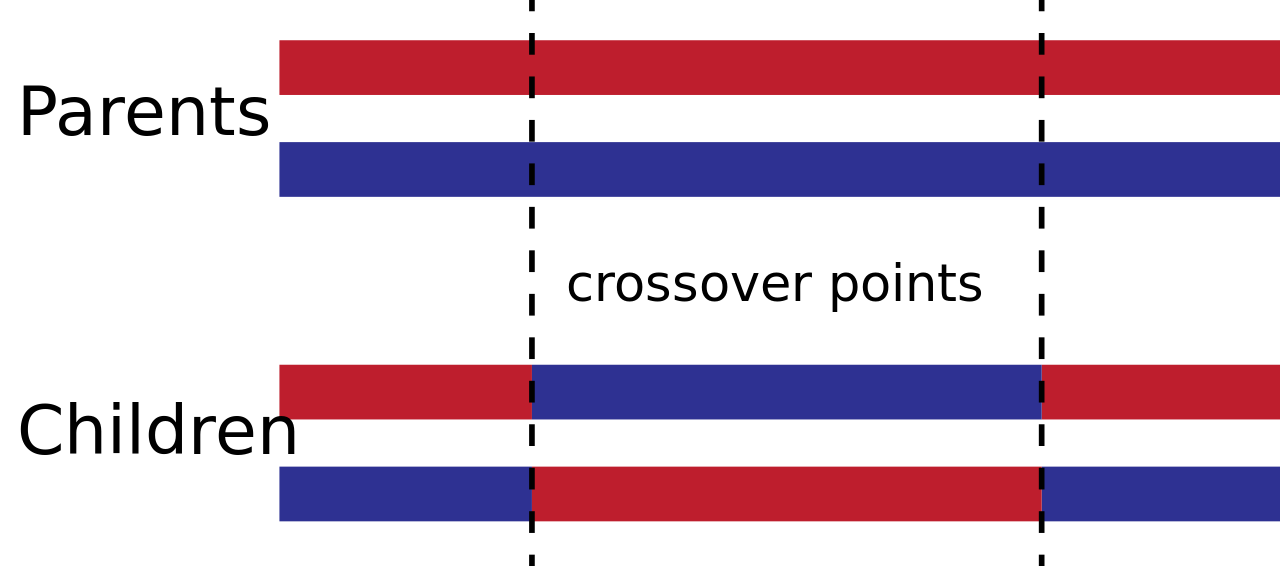
\includegraphics[scale=0.2]{2pcrossover} \\
Two-points crossover. \textit{Source: Wikipedia}
\end{center}
The best solution $X^*$ plays an important guiding role in this operation, which help WOA explore a new potential solution as an offspring. Apart from this, the randomly chosen solution $Y$ keeps maintaining the diversity of population and enhancing exploitation. For implementing $Crossover$ operation, see the detail in \textbf{Algorithm 3}. \\ \\
\begin{algorithm}[H]
\SetAlgoLined
 Initialize the whales population $X = \left\{X_i| i = 1, 2, ..., n\right\}$ within $[x_{min}, x_{max}]^D$ randomly. \\
 Calculate fitness of each solution (whale) \\
 $X^*\gets$ the best solution \\
 \For{$Iteration\gets0$ to $Iteration_{max}$}
 {
 	Begin updating positions: \\
 	\For{whale in population}
 	{
		Update parameters $a, A, C, l, p_1$ and $p_2$; \\ 	
		\eIf {$p_1 < 0.5$}
		{
			\eIf{$|A| < 1$}
			{
				Shrinking encircling mechanism based on Levy-Flight;\\
			}
			{	
				Search for prey (exploration phase);\\
			 
			}
		}
		{
			\eIf{$p_2 < 0.6$}
			{
				Updating by Crossover; \\
			}
			{
				Spiral updating position; \\
			}
		} 	
 	}
 	Evaluate population: fix if any solutions go beyond the boundary;\\
 	Recompute the fitness of all solutions;\\
 	Check and update $X^*$ if a better solution is found. \\
}
 	
 \KwResult{$X^*, f(X^*)$}
 \caption{Modified Whale Optimization Algorithm (MWOA)}
\end{algorithm}
\subsection{Improved Galactic Swarm Optimization}
\begin{algorithm}[H]
\SetAlgoLined
 initialization: $x_j^{(i)}$, $v_j^{(i)}$, $p_j^{(i)}$, $g_j^{(i)}$, within $[x_{min}, x_{max}]^D$ randomly. \\
 initialization: $v^{(i)}, p^{(i)}, g$ within $[x_{min}, x_{max}]^D$ randomly. \\
 \For{$Iteration\gets0$ to $Iteration_{max}$}
 {
 	Begin PSO: Level 1 \\
	\For{$i\gets1$ to $M$}
	{
		\For{$k\gets0$ to $L_1$}
		{
			\For{$j\gets1$ to $N$}
			{
				$v_j^{(i)}\gets\omega_1v_j^{(i)} + c_1r_1(p_j^{(i)} - x_j^{(i)}) + c_2r_2(g^{(i)} - x_j^{(i)})$; \\
				$x_j^{(i)}\gets$ $x_j^{(i)} + v_j^{(i)}$; \\
				\If {$f(x_j^{(i)}) < f(p_j^{(i)})$}
				{
					$p_j^{(i)}\gets$ $x_j^{(i)}$; \\
					\If {$f(p_j^{(i)}) < f(g^{(i)})$}
					{
						$g^{(i)}\gets$ $p_j^{(i)}$;
					}
				}
			}
		}
	}
	Begin MOWA: Level 2 \\
	Initialize Swarm $y^{(i)} = g^{(i)}: i = 1, 2, ..., M;$ \\
	\For{$k\gets0$ to $L2$}
	{
		\For{$i\gets1$ to $M$}
		{
			Update parameters $a, A, C, l, p_1$ and $p_2$; \\ 	
			\eIf {$p_1 < 0.5$}
			{
				\eIf{$|A| < 1$}
				{
					Shrinking encircling mechanism based on Levy-Flight;\\
				}
				{	
					Search for prey (exploration phase);\\
			 
				}
			}
			{
				\eIf{$p_2 < 0.6$}
				{
					Updating by Crossover; \\
				}
				{
					Spiral updating position; \\
				}
			}
			Evaluate population: fix if any solutions go beyond the boundary;\\
 			Recompute the fitness of all solutions;\\
 			Check and update $g$ if a better solution is found. \\			
		}
	} 	
 }
 \KwResult{$g, f(g)$}
 \caption{Modified Galactic Swarm Optimization (MGSO)}
\end{algorithm}
\end{document}
